%
Als ersten Schritt der digitalen Signalverarbeitung wollen wir uns den Übergang von einem analogen Signal zu einem digitalen näher ansehen.
Intuitiv können wir diesen Vorgang in vielen Anwendungen beobachten.
Wir nehmen im Tonstudio mit einem Mikrofon Ton auf und eine Soundkarte wandelt das analoge Signal in einen zeitdiskreten und quantisierten WAV-Datenstrom um.
In einer Fotokamera, trifft ein Feld von Lichtstrahlen ein und wird von einem \gls{cmos}-Sensor \q{direkt} abgetastet und in diskrete Helligkeitswerte pro Farbkanal umgewandelt.
Eine Antenne wandelt ein anliegendes elektro-magnetisches Feld in eine Spannung um, welche nachträglich von einem \gls{adc} abgetastet und quantisiert wird.

Mathematisch modellieren wir analoge Signale $s_a : D \rightarrow B$ meist mit $D = B = \R$.
Die Wandlung von analog zu digital transformiert dieses Signal in eine Funktion $s: \Z \rightarrow Q$ um, wobei nun $\Abs{Q} < \infty$ gilt.
Das heißt, dass das Signal nach AD-Wandlung nur noch endlich viele Werte (aus $Q$) auf einer diskreten Menge an Punkten (auf $\Z$) annehmen kann.
Meistens folgt schließlich noch ein Kodierungsschritt, der die Werte in $Q$ in eine Folge von Bits transformiert.
Wir werden uns zunächst nur mit der Diskretisierung in Zeit befassen, weil es einfach einfacher ist und die Quantisierung später in \Cref{sec:random:quanti} damit befassen.
Das heißt, dass wir uns vorstellen, dass das diskretisierte Signal nur an einer diskreten Menge an Punkten noch Informationen über das abgetastete Signal beinhaltet, wobei hier aber explizit $Q = \R$.
Weiterhin sind wir nicht an der physikalischen Umsetzung von \glspl{adc} interessiert, sondern höchstens an deren systemtheoretischer Modellierung.

Die zentralen Fragen sind nun:
\begin{itemize}
    \item Wie muss der Vorgang der Abtastung gestaltet sein, dass keine Information verloren geht?
    \item Wie können wir die Eigenschaften des analogen Signals in dessen abgetasteter Version wiederfinden?
    \item Wie können wir eine Intuition für den Vorgang der Abtastung entwickeln?
\end{itemize}
%
\subsection{Frequenz von Signalen}
%
\subsubsection{Zeit-Kontinuierliche Sinussignale}
%
Meistens werden wir uns in der Vorlesung mit reell- oder komplexwertigen Zeitsignalen befassen, d.h. wir modellieren unsere Signale als $x_a : \R \rightarrow \R$ oder $x_a: \R \rightarrow \C$.
Wobei physikalische Signale natürlich nur reellwertig sind, doch manchmal ist die Darstellung als komplexwertige Funktion besser handhabbar, siehe \eqref{complex_baseband}.
Das heißt, dass die Abtastung im Zeitbereich vonstatten geht, was sofort den Begriff der \emph{Frequenz} auf den Plan ruft, da Frequenz mit Einheit $1/[s]$ eng mit Zeit $[s]$ verknüpft ist.

Betrachten wir also erst einmal, welchen Einfluss Abtastung auf Signale mit einzelnen Frequenzen hat, am Beispiel von
%
\begin{equation}\label{eq:analog_cosine}
    x_a(t) = A \cos(\Omega t + \theta),
\end{equation}
%
wobei wir hier $A \in \R$ als Amplitude, $\Omega \in \R^+_0$ als Kreisfrequenz $\SI{1}{\radian\per\second}$, $t \in \R$ als Zeit $\SI{1}{\second}$ und die Phase $\theta \in \R$ mit Einheit $\SI{1}{\radian}$ nutzen.
Alternativ können wir auch zur Frequenz $F \in \R$ $\SI{1}{\per\second} = \SI{1}{\hertz}$ übergehen.
Dann erhalten wir
\[
x_a(t) = A \cos(2 \pi F t + \theta).
\]
Diese Funktion ist in \cref{fig:analog_cosine} dargestellt.
Wir sehen, dass die Funktion periodisch ist mit Periode $T_p = 1/F$.

\myemph{Das heißt, dass $x_a(t + k \cdot T_p)$ für $k \in \Z$ nicht vom Signal $x_a(t)$ zu unterscheiden ist!}
Also gilt
\[
x_a(t) = x_a(t + k \cdot T_p) \Text{für alle} k \in \Z, t \in \R.
\]

\begin{figure}[t]
    \begin{center}
        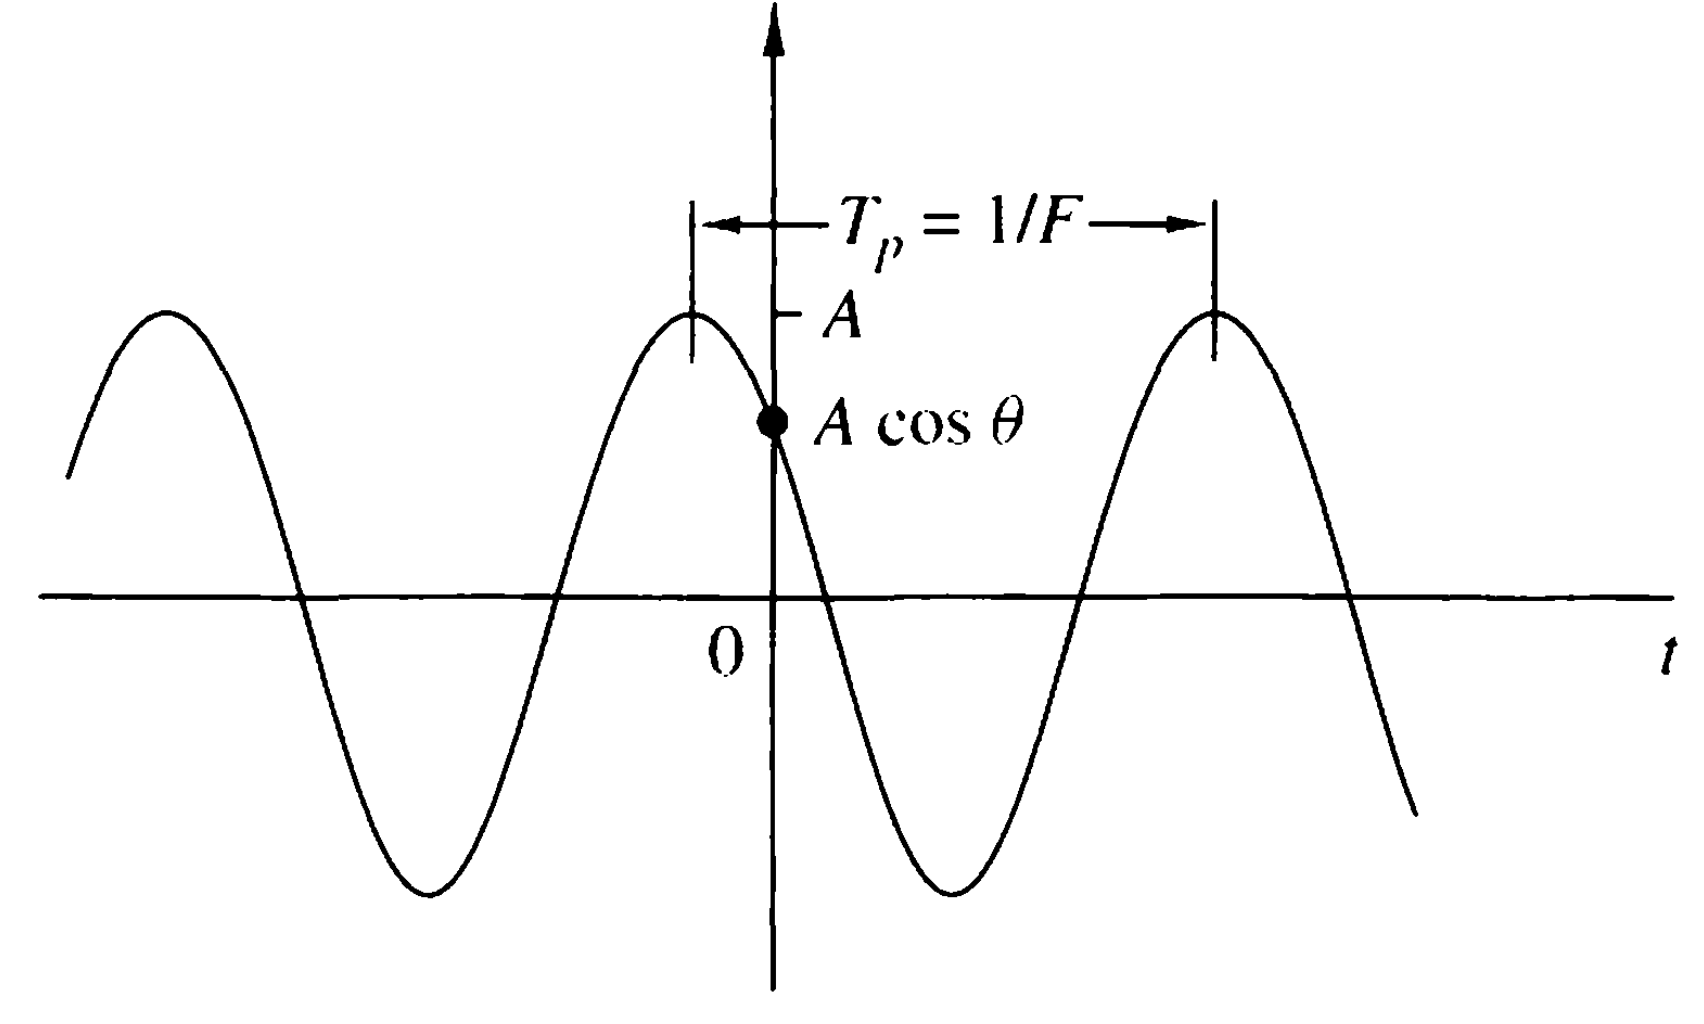
\includegraphics[width=0.48\textwidth]{img/sampling/analog_cosine.png}
        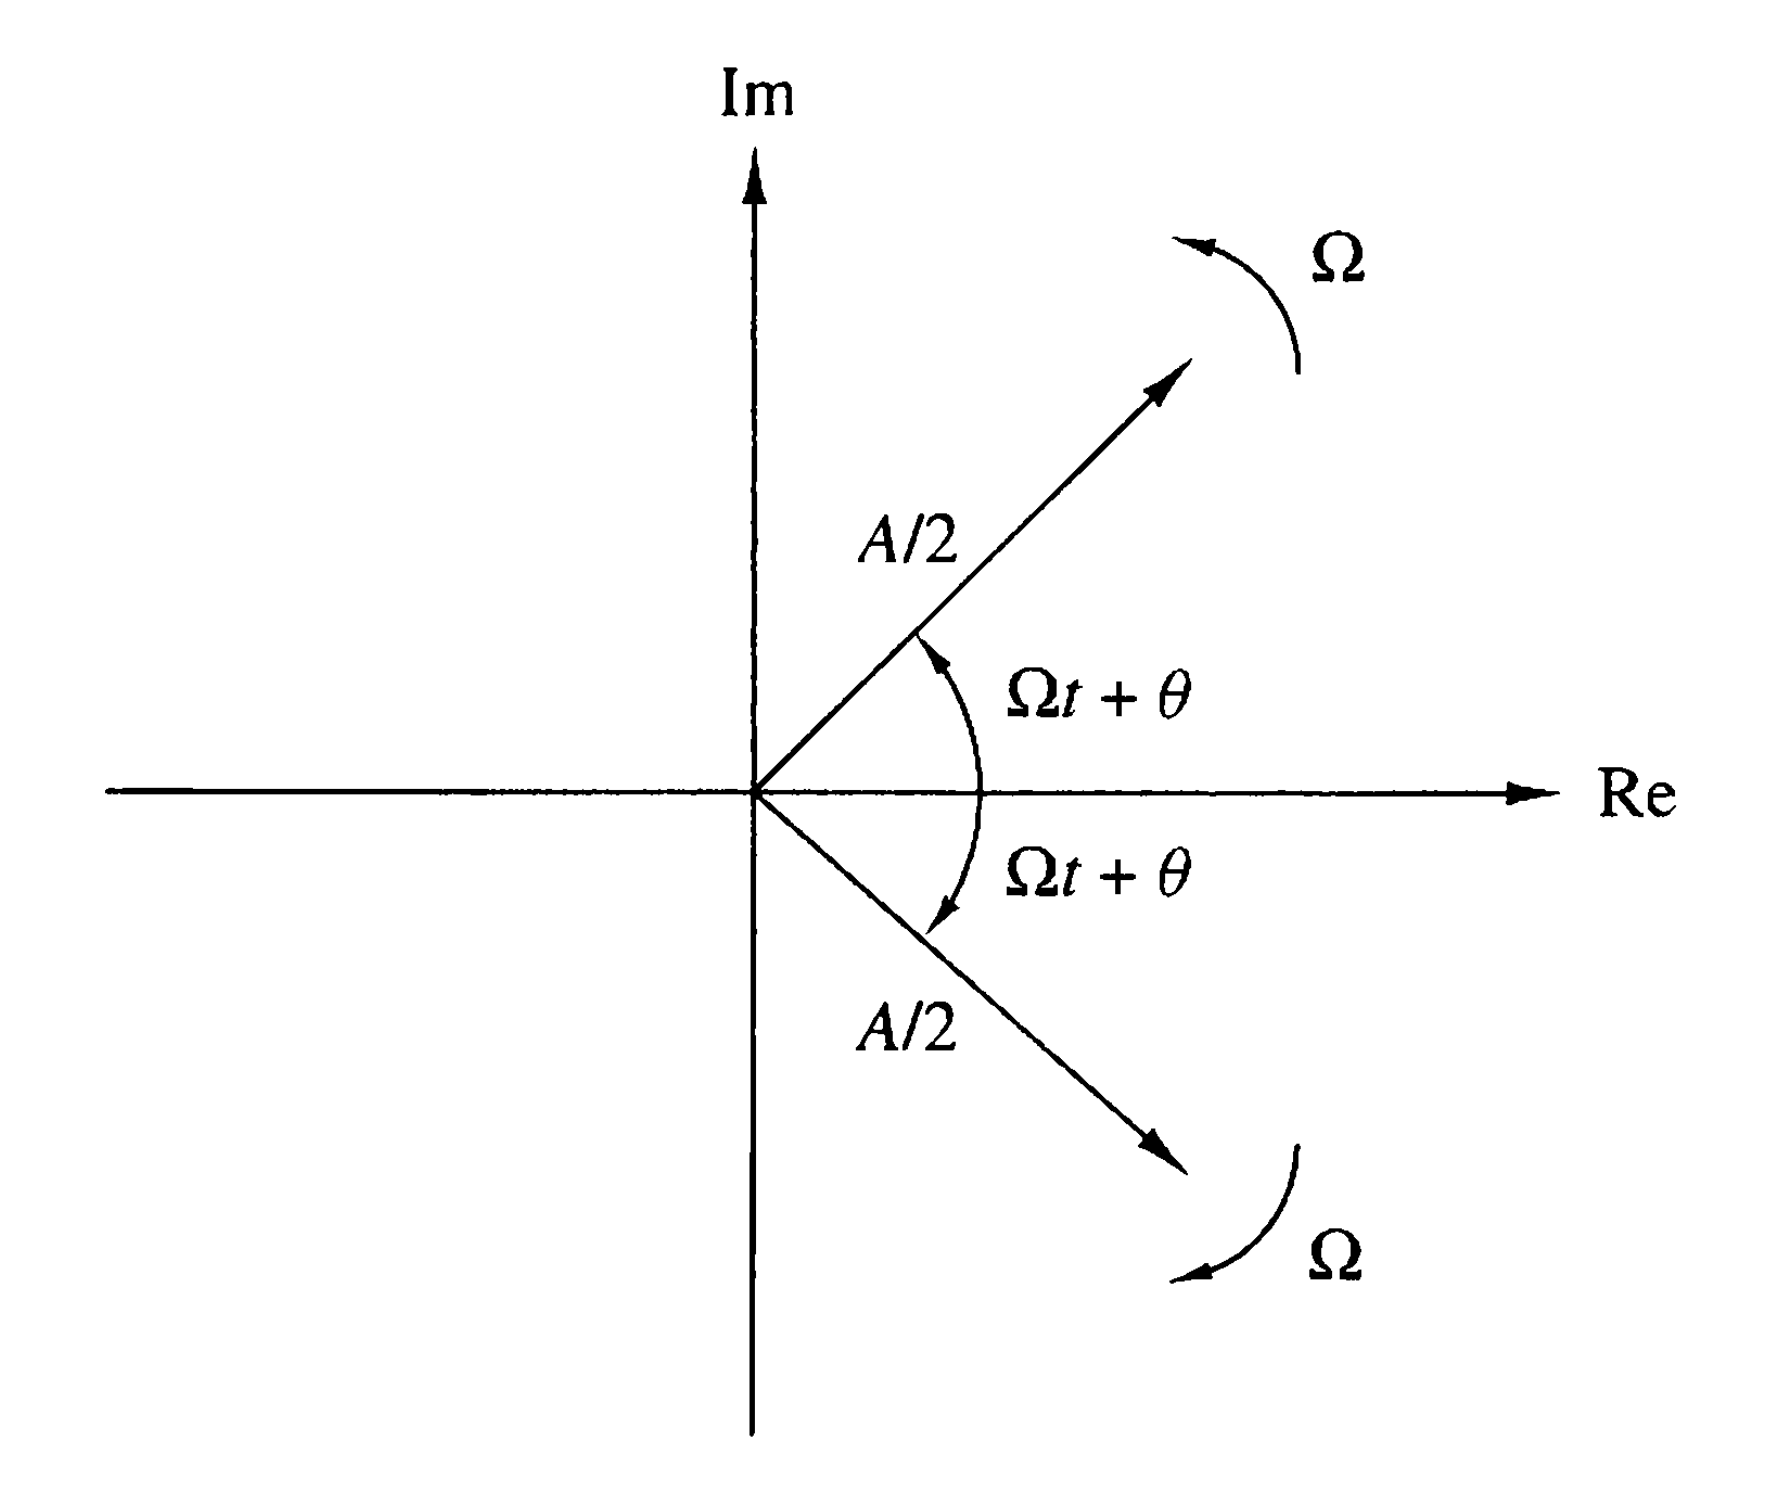
\includegraphics[width=0.48\textwidth]{img/sampling/two_phasors.png}
    \end{center}
    \caption{$x_a(t) = A \cos(2 \pi F t + \theta)$, Quelle: \cite{proakis2013}}\label{fig:analog_cosine}
\end{figure}
%
Es gibt noch eine alternative Darstellung von der obigen Funktion durch die Addition von zwei zueinander konjugierten \emph{Phasoren} als
\[
    x_a(t) 
        = A \cos(2 \pi F t + \theta) 
        = \frac A2 \exp(\jmath (\Omega t + \theta)) 
            + \frac A2 \exp(- \jmath (\Omega t + \theta)).
\]
Da die beiden überlagerten Phasoren so interpretiert werden können als rotierten diese in gegensätzliche Richtungen, ist es gerechtfertigt der physikalischen Intuition entgegen auch von \q{negativen} Frequenzen zu sprechen.
Wir erlauben also $F \in \R$, womit auch der Spezialfall $T_p = \infty$, also $x_a(t) = A$ abgedeckt ist.
Ein kleines Beispiel findet man in \Cref{py:cont_harms}.
%
\begin{listing}
    \begin{minipage}{0.49\textwidth}
        \inputminted[firstline=4]{python3}{code/cont_harms.py}
    \end{minipage}%
    \begin{minipage}{0.49\textwidth}
        \strut\vspace*{-\baselineskip}\newline
        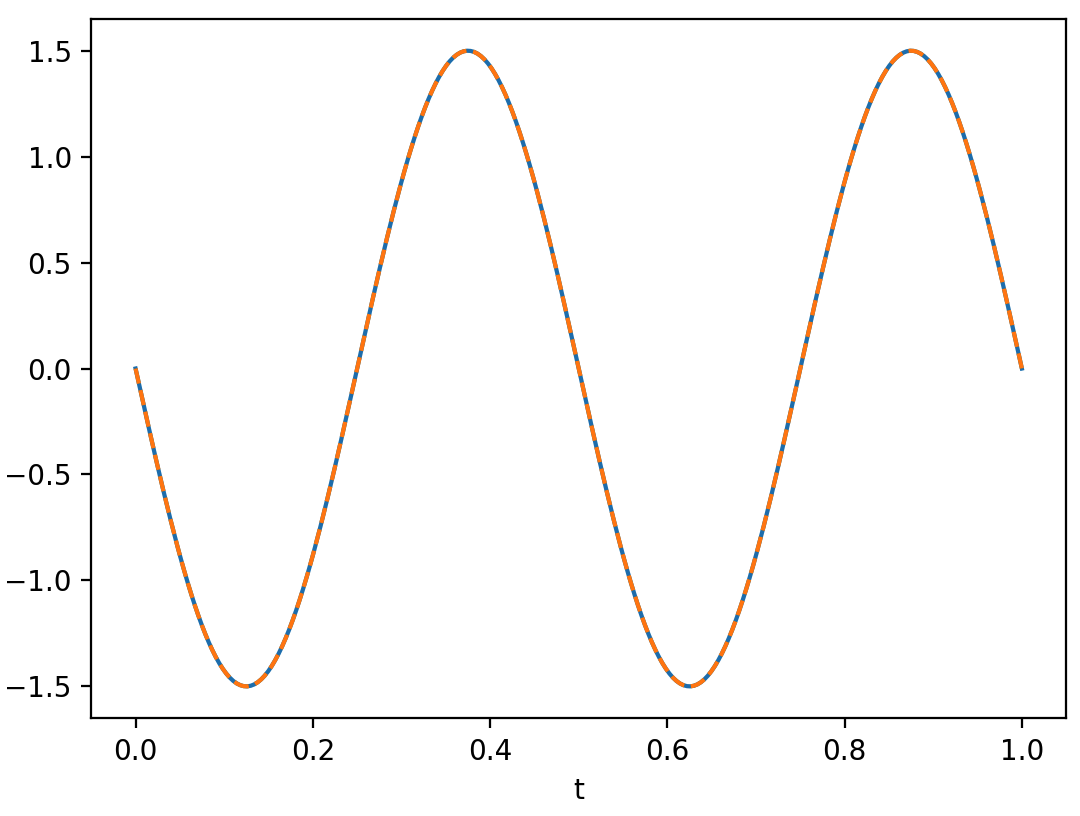
\includegraphics[width=\textwidth]{code/cont_harms.png}
    \end{minipage}
    \codecaption{dsv/code/cont_harms.py}{Berechnung und Darstellung von \eqref{eq:analog_cosine}}\label{py:cont_harms}
\end{listing}
\FloatBarrier
%
\subsubsection{Zeit-Diskrete Sinussignale}
%
Als nächstes gehen wir zu dem eigentlich interessanten Fall über, bei welchem wir von zeitdiskreten harmonischen Signalen sprechen.
Dabei gehen wir vorerst \emph{nicht} davon aus, dass das Signal durch Abtastung eines analogen/stetigen Signals entstanden ist, sondern betrachten es ganz losgelöst für sich.
In Analogie zu \eqref{eq:analog_cosine} definieren wir
%
\begin{equation}\label{eq:discrete_cosine}
    x[n] = A \cos(\omega n + \theta) = A \cos(2 \pi f n + \theta).
\end{equation}
%
Wichtig bei diskreten Signalen ist, dass ihre physikalische Interpretierbarkeit nicht direkt gegeben ist, da $n \in \Z$ nur die diskreten Werte \q{nummeriert}, also \emph{einheitenlos} ist.
Deshalb hat $f \in \R$ lediglich als Einheit \q{Zyklen pro Sample}, was man auch daran sieht, dass für $f = 1$ gilt $x[n] = A \cos(2\pi n + \theta) = A \cos(\theta)$.
Es existiert nun ein wichtiger Unterschied zwischen $x[\cdot]$ von \eqref{eq:discrete_cosine} und $x_a(\cdot)$ von \eqref{eq:analog_cosine}.
Das Signal $x[\cdot]$ ist nur periodisch, falls $f$ eine rationale Zahl ist, also $f = p/q$ für $p,q \in \Z$ und $q \neq 0$. 
\emph{Wieso?}

Ein zeitdiskrtes Signal ist periodisch, falls $x[n + N] = x[n]$ für alle $n \in \Z$.
Für unser Signal in \eqref{eq:discrete_cosine} heißt das also, dass
\[
    \cos(2 \pi f n + \theta) 
        = \cos(2 \pi f (n + N) + \theta)
        = \cos(2 \pi f n + 2 \pi f N + \theta)
\]
Da $\cos$ Periode $2\pi k$ für $k \in \Z$ besitzt, muss $2 \pi f N = 2 \pi k$ gelten, also
\[
    f = \frac kN.
\]
Andersherum kann man die kleinste Periode $N$ ermitteln, indem man $f = k/N$ vollständig kürzt, sodass also Zähler und Nenner keine gemeinsamen Teiler mehr haben, und man dann den Nenner des resultierenden Bruches als $N$ setzt. 
Ein Beispiel wird in \Cref{py:disc_harms} gezeigt. 
Man kann interessante Ergebnisse erzielen, wenn man diesen Plot für $\omega=0,\pi/8,\pi/4,\pi/2$ und $\omega=\pi$ erzeugt (Übung).
%
\begin{listing}
    \noindent
    \begin{minipage}{0.49\textwidth}
        \strut\vspace*{-\baselineskip}\newline
        \inputminted[firstline=4]{python3}{code/disc_harms.py}
    \end{minipage}%
    \begin{minipage}{0.49\textwidth}
        \strut\vspace*{-\baselineskip}\newline
        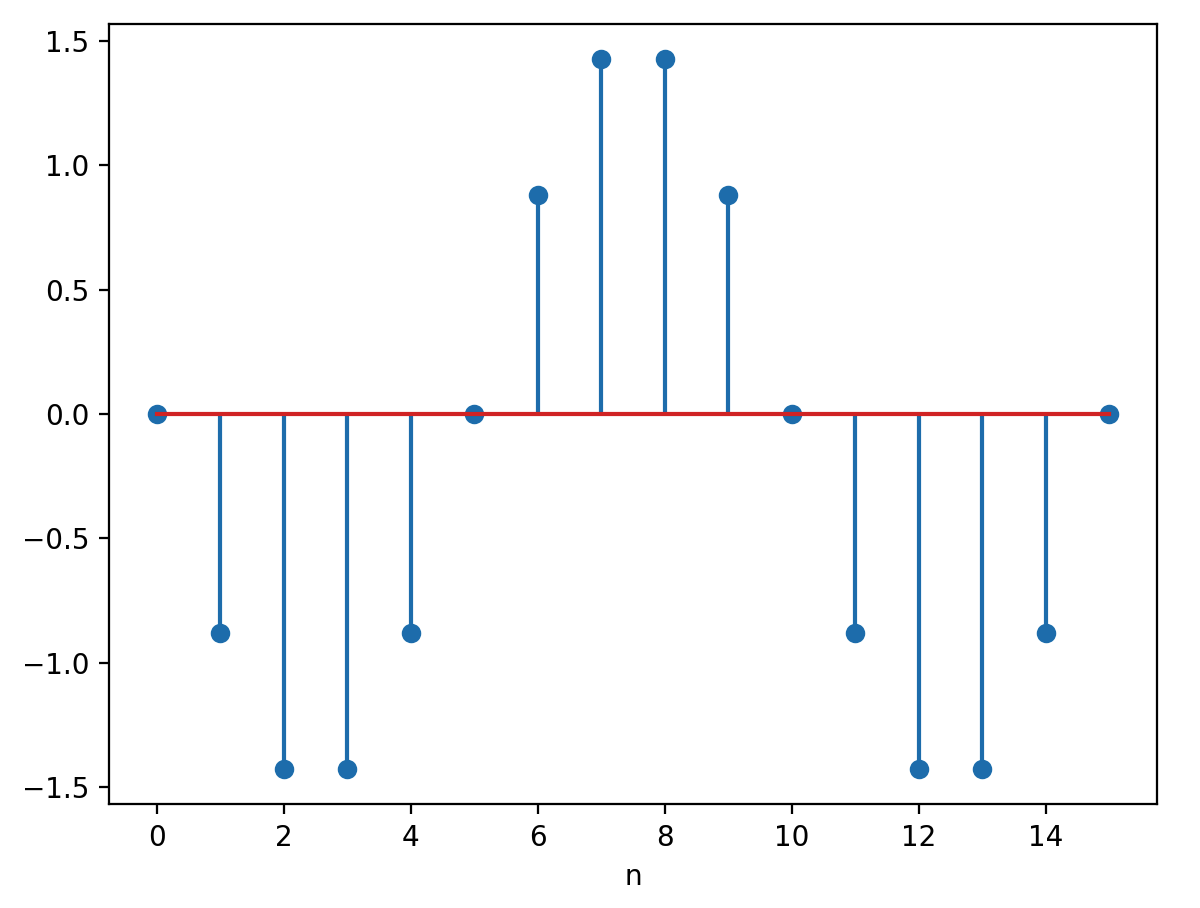
\includegraphics[width=\textwidth]{code/disc_harms.png}
    \end{minipage}
    \codecaption{dsv/code/disc_harms.py}{Berechnung und Darstellung von \eqref{eq:discrete_cosine}}\label{py:disc_harms}
\end{listing}

Die Signale der Form \eqref{eq:discrete_cosine} haben noch eine weitere wichtige Eigenschaft, die sich wieder aus der $2\pi$-Periodizität von $\cos$ ergibt. 
Betrachten wir noch einmal \eqref{eq:discrete_cosine} und wir finden, dass
\[
\cos(\omega n + \theta) = \cos(\omega n + 2\pi n + \theta) = \cos((\omega + 2\pi) n + \theta).
\]
Das heißt, dass
\[
    x[n] = \cos(\omega n + \theta) = \cos((\omega + 2\pi k) n + \theta) = x_k[n]
\]
für \emph{alle} $k \in \Z$ gilt.
Das heißt, dass sich $x_k[\cdot]$ nicht von $x[\cdot]$ unterscheiden lässt.
Man nennt dann jedes der $x_k[\cdot]$ einen \emph{Alias} von $x[\cdot]$.
Man kann deshalb auch umgekehrt sagen, dass für jedes $\omega$ mit $\Abs{\omega} > \pi$ ein zugehöriges $\omega_a$ mit $\Abs{\omega_a} < \pi$ existiert, sodass
\[
    \cos(\omega n + \theta) = \cos(\omega_a n + \theta)
\]
gilt.
Vergewissern sie sich von dieser Tatsache, indem sie verschiedene Aliase basierend auf \Cref{py:disc_harms} visualisieren (Übung).

Stellen wir uns für einen kurzen Moment vor, dass wir wissen, dass wir $x[n]$ durch Abtastung einer Funktion wie in \eqref{eq:analog_cosine} erhalten haben.
Es gilt in diesem Fall $x[n] = A \cos( 2 \pi F n \Delta T + \theta )$ für ein uns unbekanntes $F \in \R$.
Selbst wenn wir wissen, dass nur \emph{eine} Frequenz in diesem Signal vor Abtastung vorhanden war, können wir \emph{nicht} entscheiden, welche das war, da jeder Alias von $x[n]$ für die Abtastwerte von der kontinuierlichen Version in Frage kommen kann.
\emph{Es ist also nicht möglich, beliebige Signale ohne zusätzliches Vorwissen \q{einfach} abzutasten.}
%
\FloatBarrier
%
\subsection{Zeit-Kontinuierliche Komplexe Sinussignale}\label{sec:cont_complex_harm}
%
Wir wollen eine bestimmte Untermenge an Funktionen betrachten: komplexe Schwingungen, welche mit einer Frequenz $F_k$ schwingen, wobei diese Frequenz ein ganzzahliges Vielfaches einer Grundfrequenz $F_0$ ist.
Das heißt, wir betrachten also $F_k = k \cdot F_0 \Text{für} k \in \Z $ und erhalten
\[
x_k(t) = \exp(\jmath 2 \pi F_k t) = \exp(\jmath 2 \pi k F_0 t) = \cos(\jmath 2 \pi k F_0 t) + \jmath \sin(\jmath 2 \pi k F_0 t).
\]
Jedes der $x_k$ hat (wegen der Periodizität von $\cos$ und $\sin$) Periode $1/F_k = T_k = T_0/k$. 
Das heißt für wachsendes $\Abs{k}$ werden die Perioden immer um ein Vielfaches kürzer. 
Umgekehrt besitzen immernoch alle $x_k$ gemeinsame Periode, $T_0$, da für jedes $k$ gilt, dass $T_k \cdot k = T_0$.
Wir haben auch (noch) kein Problem mit Aliasing zwischen den $x_k$, da bei kontinuierlichen Signalen gilt, dass $x_{k_1} \neq x_{k_2}$, falls $k_1 \neq k_2$.

Wie wir in \Cref{sec:signals_vec} gesehen haben, können wir beliebige Linearkombination aus Signalen bilden und erhalten wieder ein Signal.
Wir können also für eine Folge von $c_k \in \C$ die Linearkombination der $x_k$ bilden und erhalten
%
\begin{equation}\label{eq:cont_fourier_series}
    x_a = \Sum{k \in \Z}{}{c_k x_k} : \R \rightarrow \C
    \Text{mit} 
    t \mapsto x_a(t) = \Sum{k \in \Z}{}{c_k x_k(t)}
        = \Sum{k \in \Z}{}{c_k \exp(\jmath 2 \pi k F_0 t)}.
\end{equation}
%
Die erste Schreibweise ist absichtlich ohne das Argument $t$, um zu verdeutlichen, dass Signale \emph{wirklich} als eigenständige Vektoren werden können und dass $x_a(t) \in \C$ \q{nur} die Auswertung von $x_a$ an der Stelle $t$ ist, welche \emph{strikt} von dem \emph{Vektor} $x_a$ zu unterscheiden ist.

Natürlich ist \eqref{eq:cont_fourier_series} als Fourier-Reihe von $x_a$ bekannt, und die $c_k$ sind die Fourierkoeffizienten von $x_a$.
Wie in \Cref{sec:signals_vec} können wir also die $c_k$ durch die Fourier-Reihe in \eqref{eq:cont_fourier_series} mit $x_a$ \emph{identifizieren}, und uns die $c_k$ somit eine alternative Darstellung von $x_a$ liefern.
Es ist hier zu beachten, dass ein \q{kontinuierliches} Objekt, also $x_a$, durch eine Menge von diskreten Werten \emph{vollständig} beschrieben wird!
%
%
%
%
\subsection{Zeit-Diskrete Komplexe Sinussignale}\label{sec:sampling:disc_sin}
%
Analog zu \Cref{sec:cont_complex_harm}, wollen wir uns Eigenschaftern zeit-diskreter komplexer Schwingungen herleiten, die von einer bestimmten Grundfrequenz $f_0$ definiert werden.
Da wir, im Unterschied zum kontinuierlichen Fall, nicht für alle $f \in \R$ eine periodische Funktion erhalten würden, wählen wir $f_0 = 1/N$ für ein $N \in \N$. 
Die Intension ist, dass wir im Falle von Frequenz $f_0$ $1/N$ Perioden pro Abtastwert erhalten werden. 
Umgekehrt wird die Schwingung mit Frequenz $f_0$ genau Periodenlänge von $N$ Samples/Abtastwerten haben.
Dann definieren wir für $k \in \Z$ die Signale $x_k[\cdot]: \N \rightarrow \C$ als
%
\begin{equation}\label{eq:disc_harms_comp}
    x_k[n] = \exp\left(
        \jmath 2 \pi k f_0 n
    \right).
\end{equation}
%
Man sieht nun leicht, dass $f_k = k/N$ immer eine rationale Zahl ist und $x_k[\cdot]$ Periodenlänge $N/k$ hat, falls $k/N \in \Z$.
Dies ist in \Cref{py:disc_harms_comp} dargestellt.

Außerdem findet man wieder, dass $x_k[\cdot]$ ein Alias von $x_{k+N}[\cdot]$ sein muss, denn mit $f_0 = 1/N$ ergibt sich
\[
 x_{k+N}[n] = \exp\left(
        \jmath 2 \pi (k + N) f_0 n
    \right)
    = \exp\left(
        \jmath 2 \pi \frac{k + N}{N} n
    \right)
    = \exp\left(
        \jmath 2 \pi \frac{k}{N} n
    \right) 
    \exp\left(
        \jmath 2 \pi \frac NN n
    \right) 
    = x_k[n].
\]
Das heißt, dass nur $N$ verschiedene $x_k[\cdot]$ existieren, wenn man diese mit Grundfrequenz $f_0 = 1/N$ definiert.
Normalerweise nimmt man jene $x_k[\cdot]$ für $k = 0, 1, \ldots, N-1$.
%
\begin{listing}
    \noindent
    \begin{minipage}{0.49\textwidth}
        \strut\vspace*{-\baselineskip}\newline
        \inputminted[firstline=4]{python3}{code/disc_harms_comp.py}
    \end{minipage}%
    \begin{minipage}{0.3\textwidth}
        \strut\vspace*{-\baselineskip}\newline
        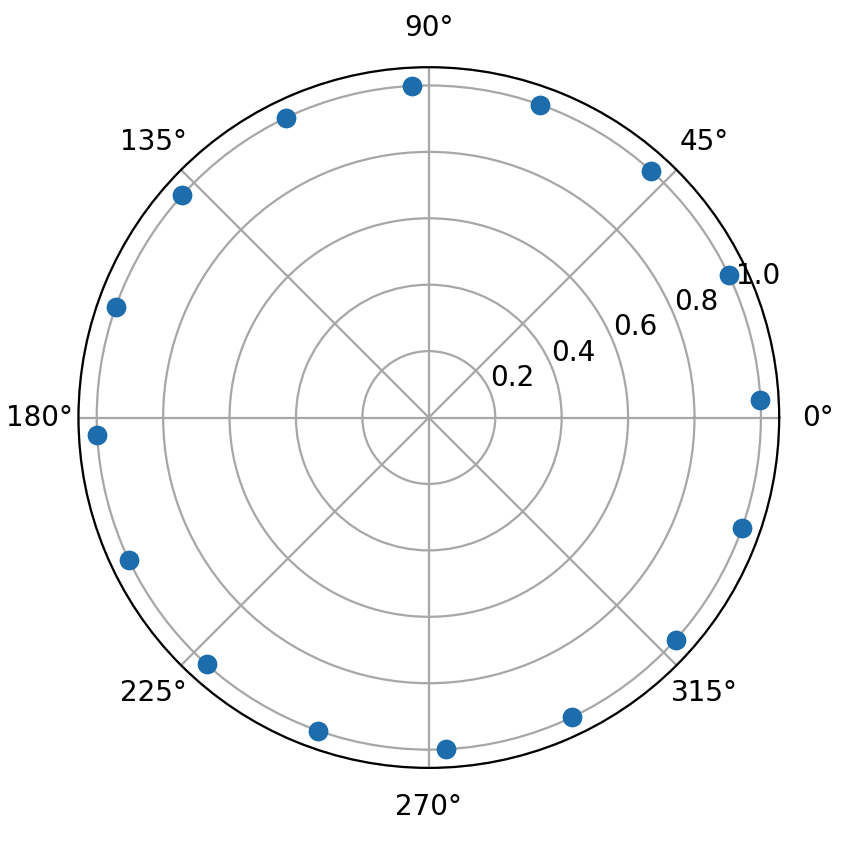
\includegraphics[width=\textwidth]{code/disc_harms_comp.png}

        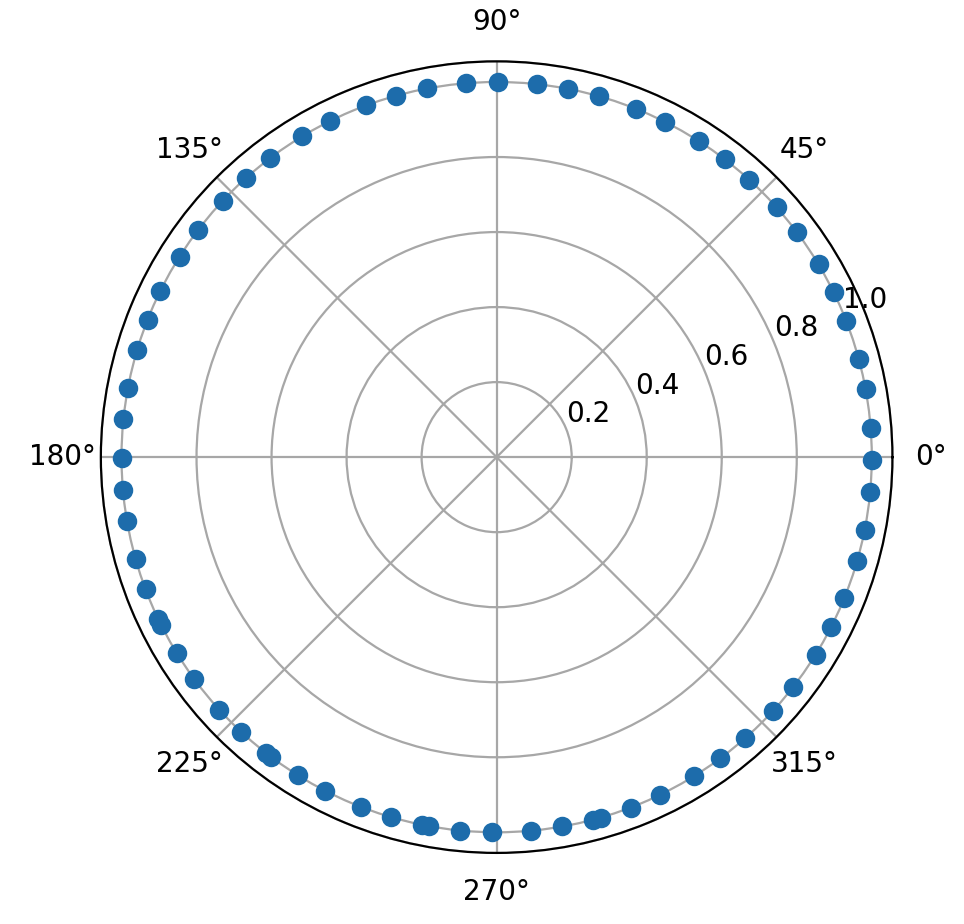
\includegraphics[width=\textwidth]{code/disc_harms_comp_e.png}
    \end{minipage}
    \codecaption{dsv/code/disc_harms_comp.py}{Berechnung und Darstellung von \eqref{eq:disc_harms_comp} für $f_0 = 1/16$ und $f_0 = 1/(5 e)$}\label{py:disc_harms_comp}
\end{listing}

Nun können wir auch wieder, wie in \eqref{eq:cont_fourier_series} eine Linearkombination der $x_k[\cdot]$ bilden.
Man beachte, dass in diesem Fall die Summation natürlich \emph{endlich} sein wird, da wir nur $N$ verschiedene $x_k[\cdot]$ zur Verfügung haben.
Wir bilden also wieder eine Linearkombination von den Vektoren $x_k[\cdot]$ durch
\[
    x[\cdot] = \Sum{k = 0}{N-1}{c_k x_k[\cdot]}
\]
und erhalten so ein Signal mit Werten
\begin{equation}\label{eq:disc_fourier_series}
    x[n] 
        = \Sum{k = 0}{N-1}{c_k x_k[n]} 
        = \Sum{k = 0}{N-1}{
            c_k \exp\left(
                \jmath 2 \pi \frac{k}{N} n
            \right) 
        },
\end{equation}
was die Fourier-Reihe eines diskreten und periodischen Signals darstellt, wobei in diesem Fall der Vektor $\bm c = [c_k]_{k=0}^{N-1} \in \C^N$, der die Koeffizienten in der Fourier-Reihe enthält, eine alternative Repräsentation des Signals ist.

Das Signal $x[\cdot]$ selbst ist periodisch mit Periodenlänge $N$, d.h. das Signal ist durch die Werte $\bm x = [x[n]]_{n=0}^{N-1} \in \C^N$ \emph{vollständig} definiert. 
Das heißt, wir können das Signal $x[\cdot]$ mit dem \emph{endlich-dimensionalen} Vektor $\bm x \in \C^N$ mit $\bm x_n = x[n]$ identifizieren.
Da genauso jedes der $x_k[\cdot]$ auch Periodenlänge $N$ hat, erhalten wir auf die gleiche Weise Vektoren $\bm x_k \in \C^N$ mit $(\bm x_k)_n = x_k[n]$.
Mit diesen endlich-dimensionalen Vektoren sind wir nun in der Lage die Fourier-Reihe in \eqref{eq:disc_fourier_series} mit \q{normalen} Vektoren durch
%
\begin{equation}\label{eq:disc_fourier_lincomb}
    \bm x = c_1 \bm x_1 + c_2 \bm x_2 + \ldots + c_{N-1} \bm x_{N-1}
\end{equation}
%
auszudrücken.
Wir sehen also wieder \emph{direkt}, dass Signale wirklich wie Vektoren behandelt werden können.

\Cref{eq:disc_fourier_series} kann auch als Abbildung $M : \C^N \rightarrow \C^N$ interpretiert werden, da wir in die rechte Seite von \eqref{eq:disc_fourier_series} einfach ein $\bm c \in \C^N$ stecken können und wir erhalten das entsprechende $\bm x = M(\bm c)$.
Noch weiter ist die Abbildung $M$ sogar linear, da 
\[
    M(\bm c^1 + \bm c^2)
        =  \Sum{k = 0}{N-1}{
            (c^1_k + c^2_k) \exp\left(
                \jmath 2 \pi \frac{k}{N} n
            \right) 
        }
        =  \Sum{k = 0}{N-1}{
            c^1_k \bm x_k
        }
        + \Sum{k = 0}{N-1}{
            c^2_k \bm x_k 
        }
        = M(\bm c^1) + M(\bm c^2).
\]
Das heißt, dass es auch eine \emph{Matrix} $\bm M \in \C^{N \times N}$ geben muss, welche uns einfach $\bm c$ in $\bm x$ umtransformiert, indem wir $\bm x = \bm M \cdot \bm c$ als Matrix-Vektor-Produkt berechnen.
Wenn wir \eqref{eq:disc_fourier_lincomb} genau betrachten sehen wir, dass wir die Matrix $\bm M$ bilden können, indem wir deren $k$-te Spalte $\bm M_{\cdot, k}$ gleich $\bm x_k$ setzen.
Wenn wir noch sicher sein könnten, dass $\bm M$ invertierbar ist, könnten wir sogar aus $\bm x$ via $\bm c = \bm M^{-1} \cdot \bm x$ die Fourierkoeffizienten $\bm c$ direkt aus einem gegebenen $N$-periodischen Signal $x[\cdot]$ bestimmen.

Wir haben hier eine sogenannte Isomorphie zwischen abgetasteten Summen von komplexen Schwingungen mit Grundfrequenz $1/N$ und dem Vektorraum $\C^N$ geschaffen.
Dies hat zur Folge, dass eine Darstellung eines solchen diskreten Signals \q{in beiden Welten} leben kann. 
In der Welt der Abtastwerte $x[n]$, als auch in der Welt der Koeffizienten $\bm c$.
%
%
%
\subsection{Abtastung von Sinussignalen}\label{sec:sample_harm}
%
Es gibt viele Möglichkeiten ein analoges Signal zu digitalisieren.
Wir beschränken uns auf Abtastung, welche ein analoges Signal auf eine regelmäßige Art und Weise \emph{direkt} auswertet.
Diese Art wird manchmal auch \q{Nyquist-Sampling} genannt, weil die theoretische Grundlage für \q{erfolgreiches} Sampling durch das Nyquist-Theorem gelegt ist.
Wir stellen uns Abtastung so vor, dass wir das Signal $x_a: \R \rightarrow \R$ direkt an gewissen Stellen beobachten können.
Wir können uns eine Art Sampling-Operator $\mathcal{S}$ vorstellen, der ein analoges Signal $x_a$ in eine abgetastete Version $x_a \mapsto \mathcal{S}(x_a)[\cdot] = x[\cdot]$ transformiert.
Durch die regelmäßige/uniforme Abtastung in Zeitabständen $T > 0$ von $x_a$ erhalten wir also
\[
    x[n] = \mathcal{S}(x_a)[n] = x_a(n T) \Text{mit} n \in \Z.
\]
Wir nennen $F_s = T^{-1}$ die Sampling-Frequenz, oder die Abtastrate.
Der Vorgang ist schematisch in \Cref{fig:uniform_sampling} dargestellt.

Da wir uns $x[\cdot]$ so vorstellen, dass es \q{einfach} eine Folge von reellen Zahlen ist, müssen wir bei der Interpretation von $x[\cdot]$ auch immer gleichzeitig im Hinterkopf behalten, dass der Wert $x[n]$ dem Wert $x_a(n T) = x_a(n/F_s)$ entspricht.
Das bedeutet, dass $t$ (als Argument von $x_a$) und $n$ (als Argument von $x[\cdot]$) durch
\[
t = n T = n/F_s
\]
miteinander in Verbindung stehen. 
Man sieht auch nun eindrucksvoll, dass dadurch $n = t \cdot F_s$ einheitenlos geworden ist, bzw.~sein muss.
%
\begin{figure}
    \begin{center}
        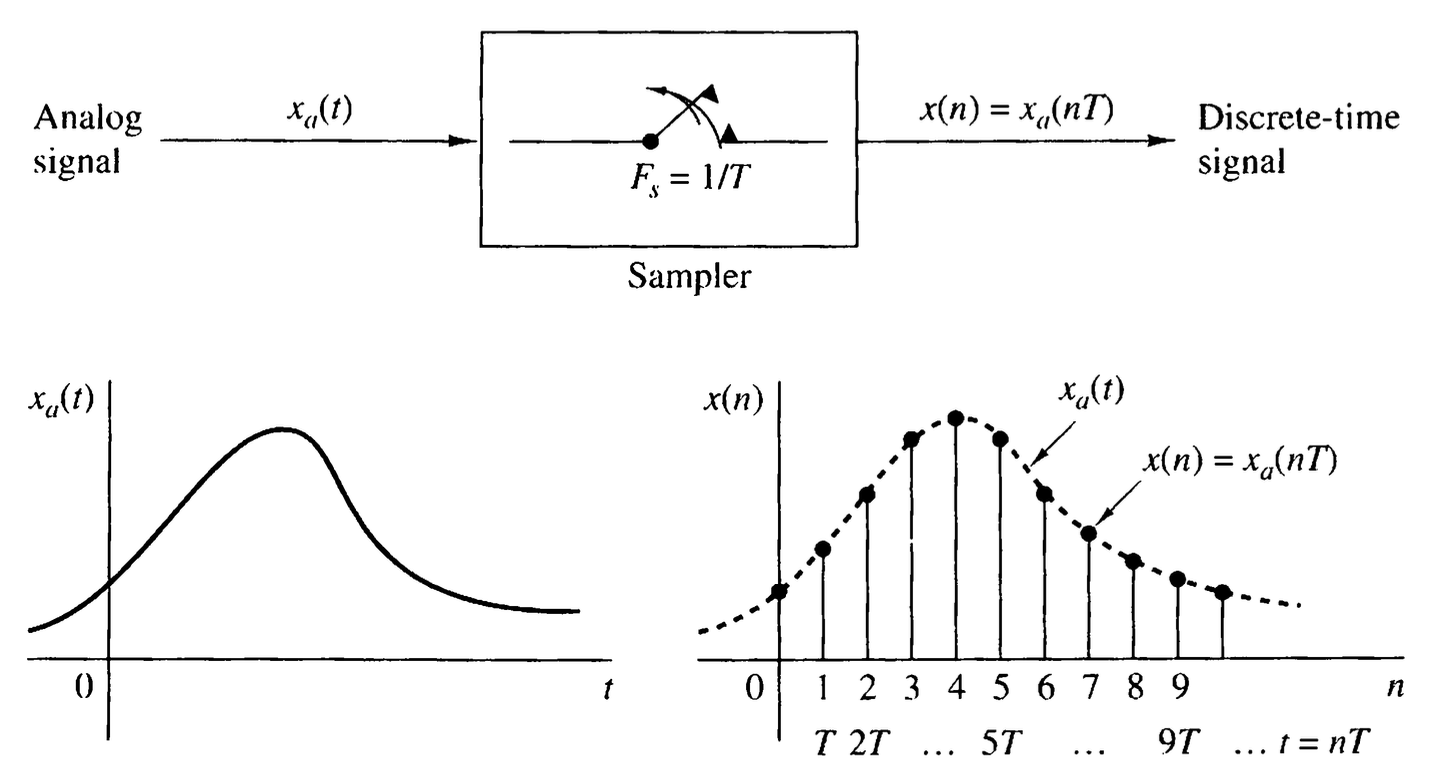
\includegraphics[width=0.7\textwidth]{img/sampling/uniform_sampling.png}
    \end{center}
    \caption{Uniforme Abtastung einer Signals. Quelle: \cite{proakis2013}}\label{fig:uniform_sampling}
\end{figure}

Weiterhin folgt aus $t = n/F_s$, dass es auch einen Zusammenhang zwischen der Frequenz $F$ einer kontinuierlichen Signals und der Frequenz $f$ im Zeit-diskreten geben muss.
Um diesen herzuleiten, betrachten wir eine einfache analoge Schwingung, wie in \eqref{eq:analog_cosine}, also
\[
x_a(t) = A \cos(2 \pi F t + \theta)
\]
und wir stellen uns vor, dass wir dieses Signal mit Samplerate $F_s = 1/T$ abtasten. Dann erhalten wir zunächst
\[
x[n] 
    = x_a(n T) 
    = A \cos(2 \pi F n T + \theta) 
    = A \cos\left(\frac{2 \pi F n}{F_s} + \theta\right).
\]
Wenn wir nun $x[n]$ in die Form von \eqref{eq:discrete_cosine} bringen, sehen wir, dass $f = F/F_s$ gelten muss.

Wie ist dies zu interpretieren? 
Wir sind mit dem analogen Signal $x_a$ gestartet, welches die Frequenz $F$ enthält.
Durch das Sampling mit Rate $F_s$ entsteht eine abgetastete Schwingung mit Frequenz $f = F/F_s$. 
Doch wir haben bereits gesehen, dass sich die Frequenz $f$ von keiner Frequenzen $f + k$ unterscheiden lässt.
Das heißt im Umkehrschluss, dass sich \emph{nach} der Abtastung die ursprüngliche Frequenz nicht eindeutig bestimmen lässt, da alle
\[
F_k = F + k \cdot F_s 
\]
bei Abtastung von $A \cos(2 \pi F_k t + \theta)$ diesselben Abtastwerte $x[n]$ ergeben würden.
Wenn wir nun also behaupten wollen, dass wir im digitalen irgendetwas sinnvolles zu tun gedenken, dann können wir dies gerade nicht so ohne weiteres.
Denn bis jetzt haben wir keine Möglichkeit das wahre analoge Signal zu rekonstruieren.
Diese missliche Lage wird in \Cref{py:aliasing} dargestellt, wo ein mögliches
$x_a$, dessen Abtastwerte $x[n]$ und zwei mögliche Aliase dargestellt sind.
Man sieht, wie die Aliase so geschaffen sind, dass auch sie Ursprung für die Abtastwerte $x[n]$ sein könnten.
%
\begin{listing}
    \noindent
    \begin{minipage}{0.49\textwidth}
        \strut\vspace*{-\baselineskip}\newline
        \inputminted[firstline=4]{python3}{code/aliasing.py}
    \end{minipage}%
    \begin{minipage}{0.49\textwidth}
        \strut\vspace*{-\baselineskip}\newline
        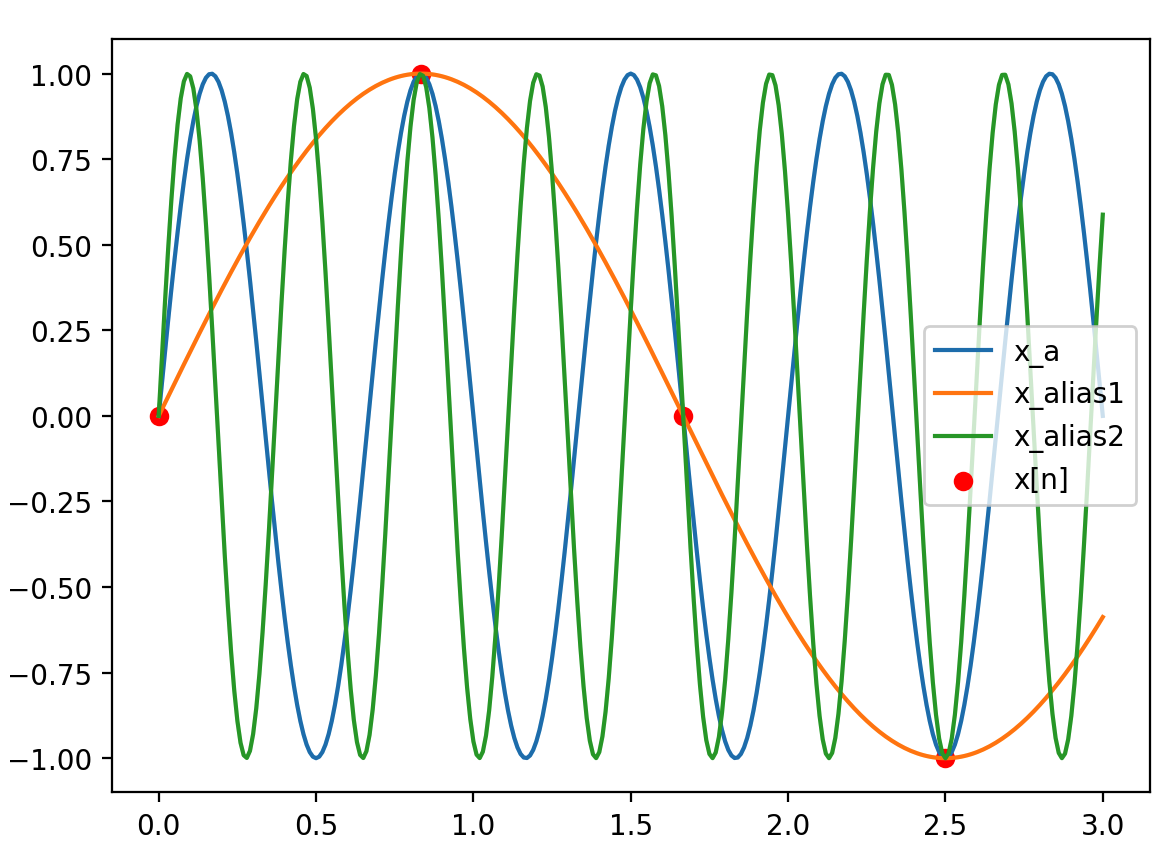
\includegraphics[width=\textwidth]{code/aliasing.png}
    \end{minipage}
    \codecaption{dsv/code/aliasing.py}{Visualisierung von $F_k = F + k \cdot F_s$}\label{py:aliasing}
\end{listing}

Die Frage ist nun, wie wir das Sampling gestalten müssen, dass wir aus $x[n]$ eindeutig das Signal $x_a$ rekonstruieren können.
In diesem Fall ist mit \q{rekonstruieren} gemeint, dass wir aus den Werten $x[n]$ den Wert $x_a(t)$ für beliebige $t \in \R$ korrekt bestimmen können.
Wie wir oben gesehen haben, ist im Digitalen nur sinnvoll von Frequenzen $f \in [-1/2,+1/2]$ zu sprechen, da wir für alle anderen $f^\prime \notin [-1/2,+1/2]$ ein $f \in [-1/2,+1/2]$ finden, das dieselben Werte in \eqref{eq:discrete_cosine} produziert.
Wegen des Zusammenhangs $f = F/F_s$ macht es also Sinn sich auch im \emph{Analogen} auf den entsprechenden Bereich zu beschränken.
Das heißt, wenn wir nur analoge Signale betrachten, bei welchen
\[
-\frac{F_s}2 \leqslant F \leqslant +\frac{F_s}2
\]
gilt, dann sind wir in der Lage aus $x[\cdot]$ das originale $x_a$ zu rekonstruieren, weil wir wissen, auf welche der Aliase wir uns beschränken müssen.

\emph{Eine Möglichkeit der perfekten Rekonstruktion von analogen mit einzelnen Frequenzen Signalen aus uniformen digitalen Abtastwerten ist die Einschränkung auf einen bestimmten Frequenzbereich.}

Umgekehrt können wir auch bei Vorwissen über die maximale Frequenz $F_{\rm max}$, also $F \in [-F_{\rm max},+F_{\rm max}]$ in einem Signal $x_a$ die Samplingrate ermitteln, sodass im Digitalen die Aliase $f + k$ für $k \neq 0$ nicht im Bereich $[-F_{\rm max},+F_{\rm max}]$ liegen.
Damit
\[
    -\frac 12 \leqslant f \leqslant + \frac 12
\]
gilt, muss also auch
\[
    -\frac 12 \leqslant \frac{F}{F_s} \leqslant + \frac 12 \Text{für alle} F \in [-F_{\rm max},+F_{\rm max}]
\]
gelten.
Deshalb muss schlussendlich $F_s > 2 F_{\rm max}$ gelten.
Es ist zu beachten, dass wir diese Überlegungen erst einmal \q{nur} für Signale der Form \eqref{eq:analog_cosine} und \eqref{eq:discrete_cosine} durchgeführt haben.
Im nächsten Abschnitt werden wir das Abtasttheorem für beliebige aperiodische Signale herleiten.
%
%
\subsection{Das Samplingtheorem}\label{sec:sampling:sampling_theorem}
%
Wir beschäftigen uns nun also allgemein mit dem Problem der Abtastung eine beliebigen analogen aperiodischen Signals $x_a$ zur Folge
\[
    x[n] = x_a(nT).
\]
Für die bequeme Analyse von kontinuierlichen Signalen und ihrem Anteil an harmonischen Komponenten, benutzen wir die \gls{ft} $\mathcal{F}$, welche ein Signal $x : \R \rightarrow \C$ transformiert in $x \mapsto \mathcal{F} x = X : \R \rightarrow \C$, wobei $X$ durch
%
\begin{equation}\label{eq:sampling:fourier_trafo}
    X(F) = \Int{-\infty}{+\infty}{x(t) \exp(-\jmath 2 \pi F t)}{t}
\end{equation}
%
definiert ist.
Wir werden versuchen, die Kombination von Klein- und Großbuchstaben $x \leftrightarrow X$ als \gls{ft}-Paar beizubehalten.
Die zugehörige inverse \gls{ft}, also die Abbildung von $X$ auf $x$ ist gegeben durch
%
\begin{equation}\label{eq:inv_fourier_trafo}
    x(t) = \Int{-\infty}{+\infty}{X(F) \exp(\jmath 2 \pi F t)}{F}.
\end{equation}

Wir wollen nun ausarbeiten, wie man diese Art Integral-Transformation rein mathematisch interpretieren kann, um eine alternative Sicht auf solche Art Transformation zu erhalten.
Betrachten wir dazu das Signal $x$ wieder als Vektor in einem Vektorraum, in dem ein \emph{Skalarprodukt} definiert ist.
Um zu erläutern, was das bringt, starten wir mit etwas Bekanntem.
Im endlich-dimensionalen Fall, also wenn $\bm x, \bm y \in \C^N$, dann ist ein mögliches Skalarprodukt $\ScPr{\cdot}{\cdot} : \C^N \times \C^N \rightarrow \R$ durch
\[
 \ScPr{\bm x}{\bm y} 
    = \Sum{i = 1}{N}{x_i \cdot y^\ast_i} 
    = y^\herm \cdot x
\]
gegeben, wobei der letzte Ausdruck das Matrix-Vektor-Produkt einer $\C^{N \times 1}$ Matrix und einem Vektor in $\C^N$ darstellt.
Man kann nun $\ScPr{\bm x}{\bm y}$ betrachten, um zu ermitteln, wie \q{ähnlich} die Vektoren $\bm x$ und $\bm y$ sind.
Beispielsweise nennen wir die beiden Vektoren orthogonal/senkrecht, falls $\ScPr{\bm x}{\bm y} = 0$. 
In diesem Fall interpretieren wir dies intuitiv so, dass $\bm x$ und $\bm y$ keine \q{gemeinsamen} Anteile haben.
Beispielsweise, wenn wir einen dritten Vektor $\bm z = \alpha \bm x + \beta \bm y$ betrachten und es gilt, dass $\ScPr{\bm x}{\bm y} = 0$, dann schlägt sich dies auch auf das Skalarprodukt von $\ScPr{\bm x}{\bm z}$ nieder, da
%
\[
    \ScPr{\bm x}{\bm z} 
        = \ScPr{\bm x}{\alpha \bm x + \beta \bm y}
        = \alpha \ScPr{\bm x}{\bm x}.
\]
%
Beim Bilden von $\ScPr{\bm x}{\bm z}$ können wir also einen etwas asymmetrischen Standpunkt einnehmen und uns vorstellen, dass wir ermitteln, wie viele \q{Anteile} von $\bm x$ in $\bm z$ zu finden sind.

Man sieht, dass dies in gewisser Weise erlaubt mit hochdimensionalen Objekten eine Art Geometrie zu betreiben.
Man kann noch weiter gehen und mit einem Skalarprodukt Korrelationen, Winkel und Längen definieren.

Wir wollen nun dieses Konzept auf kontinuierliche Signale erweitern und dann die \gls{ft} in diesem Licht interpretieren.
Man kann zeigen, dass für zwei Funktionen $x,y : \R \rightarrow \C$ die Abbildung $(x,y) \mapsto \ScPr{x}{y}$ mit
%
\begin{equation}\label{eq:cont_scpr}
    \ScPr{x}{y} = \Int{-\infty}{+\infty}{
        x(t) \cdot y^\ast(t)
    }{t}
\end{equation}
%
ein Skalarprodukt definiert. 
Auch hier halten wir an der Interpretation fest, dass wir damit berechnen, wie ähnlich sich $x$ und $y$ sind.
Definieren wir nun die Signale $k_F: \R \rightarrow \C$ durch $k_F(t) = \exp(\jmath 2 \pi F t)$, dann können wir \eqref{eq:sampling:fourier_trafo} umschreiben zu
\[
\ScPr{x}{k_F} 
    = \Int{-\infty}{+\infty}{
        x(t) \cdot \exp(\jmath 2 \pi F t)^\ast
    }{t}
    = \Int{-\infty}{+\infty}{
        x(t) \cdot \exp(-\jmath 2 \pi F t)
    }{t}
    = X(f).
\]
Dies suggeriert uns also, dass wir die \gls{ft} als Skalarprodukt von dem zu transformierenden Signal und einem geeignet gewählten Transformationskern interpretieren können.
Die Zuordnung von $F \mapsto \ScPr{x}{k_F}$ definiert dann im Grunde die Funktion $X$ für alle $F$.

Genauso erhalten wir für die Folge der Abtastwerte $x[\cdot]$ die \gls{dtft} als Skalarprodukt von $x[\cdot]$ und der Folge $k_f[n] = \exp(\jmath 2 \pi f n)$, also
%
\begin{equation}\label{eq:dtft_inner_prod}
    X(f) = \Sum{n \in \Z}{}{
            x[n] k_f[n]^\ast
        }
        = \Sum{n \in \Z}{}{
            x[n] exp(-\jmath 2 \pi f n)
        }.
\end{equation}
%
Die inverse \gls{dtft} ergibt sich durch
\[
x[n] = \Int{-1/2}{+1/2}{X(f) \exp(\jmath 2 \pi f n)}{f}.
\]
Wir haben nun alle Werkzeuge zusammen, um genauer zu Analysieren, was bei Abtastung von $x_a$ zu $x[\cdot]$ geschieht.
Wir erinnern uns, dass gilt für die Abtastpunkte gilt, dass $t = nT = n/F_s$ gilt.
Wir erhalten dann mit $x[n] = x_a(nT)$ und der inversen \gls{ft} angewandt auf $X_a$, dass
\[
x[n] = x_a(nT) = \Int{-\infty}{+\infty}{X_a(F) \exp(\jmath 2 \pi F/F_s n)}{F}
\]
gelten muss.
Setzen wir nun auch für $x[\cdot]$ die inverse \gls{dtft} ein, erhalten wir mit $f = F/F_s$ (siehe \Cref{sec:sample_harm}) als Variablentransformation, dass
\[
    \frac{1}{F_s} \Int{-{F_s}/2}{+{F_s}/2}{X(f) \exp(\jmath 2 \pi F/F_s n)}{F}
    = \Int{-\infty}{+\infty}{X_a(F) \exp(\jmath 2 \pi F/F_s)}{F}
\]
gilt. 
Wichtig ist an diesem Ausdruck, dass wir nun einen Zusammenhang zwischen der \gls{dtft} $X$ und der \gls{ft} $X_a$ gefunden haben.
Die Integration auf beiden Seiten ist auch bezüglich desselben Integrationskernes $\exp(\jmath 2 \pi \cdot/F_s n)$.
Das heißt, dass es möglich sein sollte, einen Ausdruck herzuleiten, der $X$ in Abhängigkeit von $X_a$ ausdrückt.
Mit ein wenig algebraischem Grindwork findet man
\begin{equation}\label{eq:spectrum_sampled}
    X(f) = F_s \Sum{k \in \Z}{}{
        X_a((f - k) F_s)
    }.
\end{equation}

Wie ist dies nun zu interpretieren? 
Im Grunde bestätigt \eqref{eq:spectrum_sampled} für beliebige Signale, was wir bereits für Signale mit einzelnen Frequenzen (siehe \eqref{eq:analog_cosine}) gefunden hatten.
Das Spektrum wird durch die Abtastung periodifiziert und zwar entsteht das periodische Spektrum $X$ durch Wiederholung von um $1/F_s$ gestauchte Kopien von $X_a$ mit Abstand $1/F_s$.

Andererseits kann man es auch so sehen, dass der Wert $X(f)$ sich ergibt aus Summation der Werte $X_a(f \cdot F_s - k F_s)$ für alle $k \in \Z$. 
Also an der Stelle $f$ erscheinen die Werte von $X_a$ an den Stellen $f F_s - k F_s$.
Das heißt, wie die Periodifizierung vonstatten geht h"ngt maßgeblich von der Samplingfrequenz $F_s$ ab!

Man sieht nun auch wieder schön, dass unsere obige Argumentation zum Verhältnis von Samplingfrequenz und maximaler Frequenz im Signal immernoch gilt, da nun gelten muss, dass \emph{alle} belegten Frequenzen von $x_a$ sich im Intervall $[-F_s/2,+F_s/2]$ befinden müssen, da sich sonst die Kopien von $X_a$ in \eqref{eq:spectrum_sampled} überlappen.
Dies ist äquivalent zur Forderung, dass
\[
\Abs{X_a(F)} = 0 \Text{für} \Abs{F} > F_s/2
\]
gelten muss. 
In diesem Fall spricht man davon, dass $X_a$ \emph{bandbegrenzt} ist.
Das kleinste $F \in \R$, was obige Ungleichung erfüllt, nennen wir $F_{\rm max}$.

Wir sind nun beinahe am Ziel angelangt, dass wir das Samplingtheorem formulieren können.
Wir benötigen lediglich noch eine Möglichkeit aus den Abtastwerten $x[\cdot]$ das Signal $x_a$ zu rekonstruieren.
Wenn kein Aliasing vorliegt, also $F_{\rm max} < F_s/2$, dann können wir $X_a$ aus $X$ berechnen, indem wir
\[
X_a(F) = \begin{cases}
    \frac{X(F/{F_s})}{F_s}, \Abs{F} \leqslant F_s/2, \\
    0 \Text{sonst}
\end{cases}
\]
setzen.
Wir wissen außerdem, dass sich $X$ durch die \gls{dtft} durch
\[
    X(f) = \Sum{n \in \Z}{}{
        x[n] \exp(-\jmath 2 \pi n F/F_s)
    }
\]
berechnen lässt.
Weiter können wir nun auch $x_a$ durch Integration über einen endlichen Bereich durch
\[
    x_a(t) = \Int{-F_s/2}{+F_s/2}{X_a(F) \exp(\jmath 2 \pi F t)}{F}.
\]
erhalten. 
Wir setzen nun einfach alles ein und erhalten
\[
x_a(t) = \frac{1}{F_s}\Int{-F_s/2}{+F_s/2}{
    \Sum{n \in \Z}{}{
        x[n] \exp(-\jmath 2 \pi n F/F_s)
    } 
    \exp(\jmath 2 \pi F t)}{F}.
\]
Toll, aber wir müssen dies nun noch ein wenig umformen. Zuerst vertauschen wir Integration und Summation, weil wir es dürfen und nutzen $x[n] = x_a(n/F_s)$. Dies ergibt
\[
x_a(t) = \frac{1}{F_s}\Sum{n \in \Z}{}{
            x_a(n/F_s)
            \Int{-F_s/2}{+F_s/2}{
                \exp(-\jmath 2 \pi n F/F_s)
                \exp(\jmath 2 \pi F t)
            }{F}
        }.
\]
Wir sind nicht wirklich schlauer, aber wir wissen aus unserer Erfahrung von Integration von komplexen Funktionen, dass
\[
    \frac{1}{F_s}\Int{-F_s/2}{+F_s/2}{
        \exp(-\jmath 2 \pi n F/F_s)
        \exp(\jmath 2 \pi F t)
    }{F} = \frac{\sin(\pi F_s (t - n/Fs))}{\pi F_s (t - n/F_s)} = \Sinc(F_s (t - n/Fs)).
\]
Wir nutzen nun wiederum die Interpretation von Integration eines Produktes von Funktionen als deren Skalarprodukt.
Wir bilden also das Skalarprodukt von zwei Funktionen mit Periode $F_s$, d.h. es genügt das Integral im Intervall $[-F_s/2, +F_s/2]$ zu bilden.
Sehen wir genauer hin, bilden wir also das Skalarprodukt $\ScPr{k_t}{k_{n/F_s}}$, wobei ähnlich wie oben
\[
k_t(F) = \exp(\jmath 2 \pi F t)
\]
definiert wurde.
Das heißt nun in der Sprache von Skalarprodukten, dass wir die $\Sinc$-Funktion erhalten, als
\[
    \Sinc(F_s (t - n/Fs)) = \ScPr{k_t}{k_{n/F_s}}.
\]
Wenn man es ein wenig allgemeiner Formuliert, kann man sagen, dass die $\Sinc$-Funktion nur ein spezieller \emph{Interpolationskern} ist, der sich aus der Definition von $k_t$ ergibt.
Wir werden später noch ein weiteres Beispiel für so einen Kern betrachten. Zusammenfassend für diesen \Cref{sec:sampling} steht nun folgendes
\begin{Thm}[Samplingtheorem]\label{stm:sampling_theorem}
Gegeben sei ein analoges Signal $x_a$ mit Frequezen in $[-F_{\rm max},+F_{\rm max}]$ und dessen Abtastwerte $x[\cdot]$ mit $x[n] = x_a(nT)$, wobei $T = 1/F_s$.

Falls $F_s > 2 F_{\rm max}$, dann gilt
\begin{equation}\label{eq:sampling_theorem}
    x_a(t) = \Sum{n \in \Z}{}{
        x[n] \cdot g_{F_s}(t - n T),
    }
\end{equation}
wobei der Interpolationskern $g : \R \rightarrow \R$ gegeben ist durch
\[
g_{F_s}(t) = \frac{\sin(\pi F_s t)}{\pi F_s t}.
\]
\end{Thm}

\textbf{Hinweis:} Das Samplingtheorem, wie es in \cite{proakis2013} formuliert ist, beinhaltet einen kleinen, aber entscheidenden Fehler. Die Definition des Interpolationskernes $g_F$ ist dort mit
\[
g(t) = \frac{\sin(2 \pi B t)}{2 \pi B t}.
\]
gegeben. 
Doch in diesem Falle würde der Interpolationskern von der Bandbreite des Signals $x_a$, aber nicht von der Abtastrate $F_s$ abhängen. 
Die angegebe Definition ist nur korrekt, falls $F_s = 2 B$, wir also mit der \emph{minimalen} Samplerate abgetastet haben.
In diesem Fall spricht man auch von \emph{kritischer Abtastung}.
%
\begin{listing}
    \begin{minipage}{0.49\textwidth}
        \strut\vspace*{-\baselineskip}\newline
        \inputminted[firstline=4,lastline=51]{python3}{code/sampling_theorem.py}
    \end{minipage}
    \begin{minipage}{0.49\textwidth}
        \strut\vspace*{-\baselineskip}\newline
        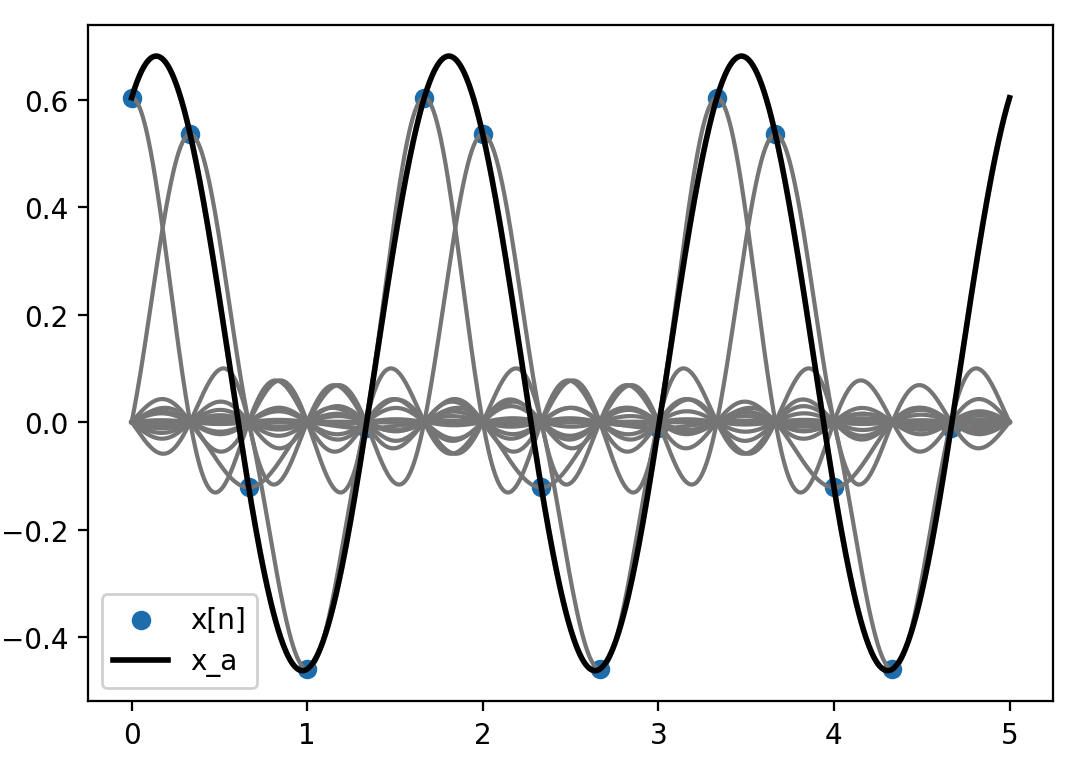
\includegraphics[width=\textwidth]{code/sampling_theorem.png}
    \end{minipage}
    \codecaption{dsv/code/sampling_theorem.py}{Berechnung und Darstellung von \Cref{stm:sampling_theorem}}\label{py:sampling_theorem}
\end{listing}

Es ist weiterhin noch zu erwähnen, dass wir genau genommen immer noch nicht wissen, wie wir überprüfen können, welche maximale Frequenz $F_{\rm max}$ von einem analogen Signal $x_a$ belegt wird.
Dies liegt daran, dass wir im Vorhinein -- also vor Abtastung -- keinen Zugriff auf das abzutastende Signal haben.
Das heißt, dass wir auch noch nicht überprüfen können, ob wir das Samplingtheorem eingehalten haben, oder einhalten werden, falls wir Abtasten sollten.
Man muss sich also für ein gegebenes System, das einem Signale produziert, die abgetastet werden sollen, auf anderem Weg überlegen, wie man die Bedingung $\Abs{X_a(F)} = 0 \Text{für} \Abs{F} > F_s/2$ überprüfen kann.

\FloatBarrier
